\documentclass[11pt,a4paper]{article}
\usepackage[utf8]{inputenc}
\usepackage{tikz}
\usepackage{hyperref}
\usepackage{geometry}
\usepackage{graphicx}
\usepackage{tcolorbox}
\usetikzlibrary{shapes.geometric, arrows, positioning}

\geometry{a4paper, margin=1in}

\title{\textbf{TruLurn Retrieval-Augmented Generation (RAG) Architecture Report}}
\author{System Architecture Documentation}
\date{\today}

\begin{document}
\maketitle

\section{Introduction}
This report provides a comprehensive overview of the Retrieval-Augmented Generation (RAG) pipeline implemented in the TruLurn platform. The pipeline ensures that the AI Teacher is securely and accurately grounded in context retrieved from course materials, user queries, and interaction history.

\section{Data Ingestion \& Chunking}
The ingestion process, primarily handled by \texttt{sources.ts}, supports various file types including Markdown (\texttt{.md}), Text (\texttt{.txt}), JSON, and CSV. 
When a user uploads materials, the system extracts the raw text. If the file is valid, the text is split into chunks (e.g., \texttt{Source: [filename] \textbackslash n [content]}). This foundational step ensures that documents are converted into a standardized format ready for processing by the embedding model.

\section{Embedding Strategy}
Once the text is extracted, it undergoes an embedding process where raw text is converted into dense numerical vectors. TruLurn uses the \texttt{gemini-embedding-001} model provided by the Gemini API.
Three main entities are embedded:
\begin{itemize}
    \item \textbf{Pages}: Course content chunks alongside their focus and summaries.
    \item \textbf{Doubt Messages}: The chat history between the user and the AI assistant to provide interaction context.
    \item \textbf{Source Chunks}: User-uploaded files containing grounded curriculum sources.
\end{itemize}

\section{Vector Storage}
The generated vector embeddings are stored in \textbf{MongoDB Atlas} using its Vector Search capabilities. 
As defined in \texttt{indexes.ts}, vector search indexes are configured for three collections: \texttt{pages}, \texttt{doubtMessages}, and \texttt{sourceChunks}.
These indexes are configured with:
\begin{itemize}
    \item \textbf{Dimensions}: 768 (standard for Gemini embeddings).
    \item \textbf{Similarity Metric}: Cosine similarity.
    \item \textbf{Metadata Filters}: Indexed on \texttt{course\_id}, \texttt{user\_id}, and \texttt{topic\_id} to ensure strict data isolation and efficient querying.
\end{itemize}

\section{Retrieval Process}
During query time, the user's question or context request is first embedded into a vector using the same \texttt{gemini-embedding-001} model. 
The \texttt{retrieval.ts} module executes a \texttt{\$vectorSearch} aggregation pipeline against MongoDB. 
\begin{enumerate}
    \item \textbf{Similarity Search}: Matches the user's query vector against stored document vectors.
    \item \textbf{Filtering}: Applies strict filters (e.g., \texttt{course\_id} and \texttt{user\_id}) to prevent data leakage across users or courses.
    \item \textbf{Context Assembly}: Collects top $K$ relevant Pages, Doubt Messages, and Source Chunks, compiling them into a unified \texttt{CourseMemoryContext}.
    \item \textbf{Fallback Mechanism}: If the vector search yields no results or fails, the system gracefully falls back to retrieving the most recent documents in the respective collections.
\end{enumerate}
This assembled context is finally passed to the Gemini LLM as part of the prompt, allowing it to generate accurate, context-aware responses without hallucinating.

\section{System Architecture Diagram}

\begin{figure}[h]
\centering
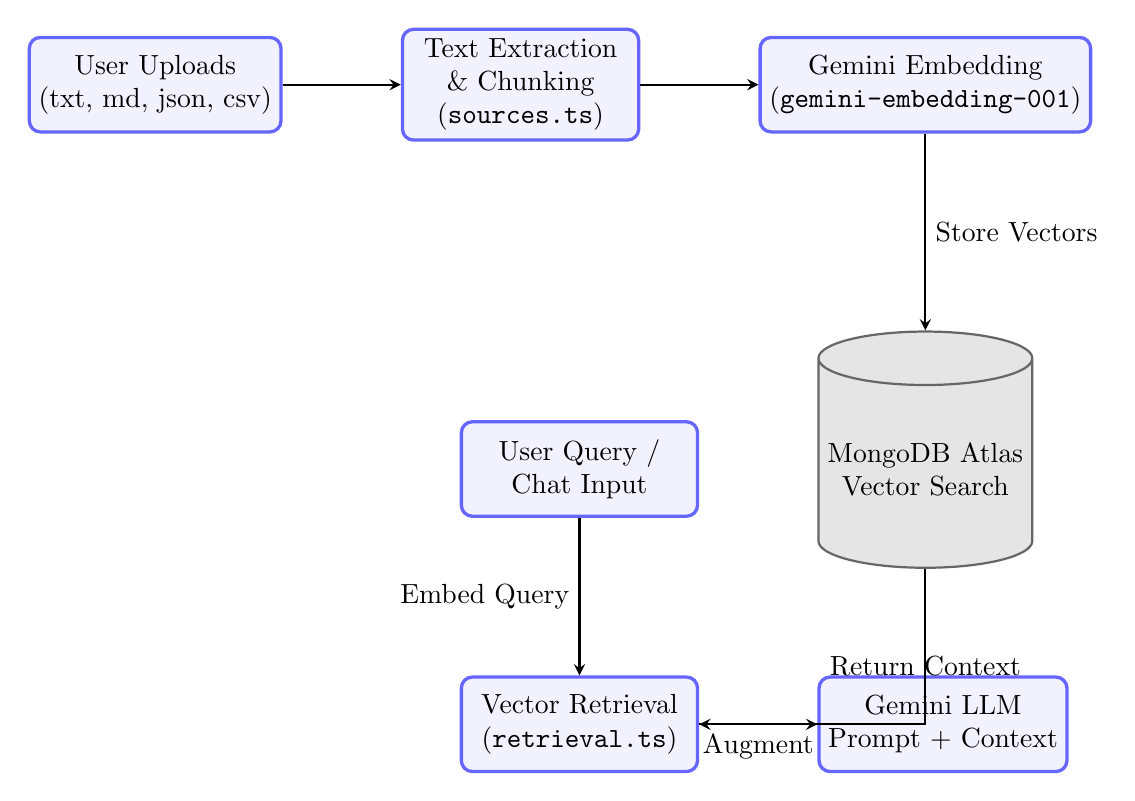
\begin{tikzpicture}[
    node distance=2cm and 1.5cm,
    box/.style={rectangle, draw=blue!60, fill=blue!5, very thick, minimum width=3cm, minimum height=1.2cm, align=center, rounded corners},
    db/.style={cylinder, draw=black!60, fill=black!10, thick, aspect=0.25, minimum width=2.5cm, minimum height=3cm, align=center, shape border rotate=90},
    arrow/.style={thick, ->, >=stealth}
]

% Nodes
\node (upload) [box] {User Uploads \\ (txt, md, json, csv)};
\node (chunking) [box, right=of upload] {Text Extraction \\ \& Chunking \\ (\texttt{sources.ts})};
\node (embedding) [box, right=of chunking] {Gemini Embedding \\ (\texttt{gemini-embedding-001})};

\node (mongo) [db, below=of embedding, yshift=-0.5cm] {MongoDB Atlas \\ Vector Search};

\node (query) [box, left=of mongo] {User Query / \\ Chat Input};
\node (retrieval) [box, below=of query] {Vector Retrieval \\ (\texttt{retrieval.ts})};
\node (llm) [box, right=of retrieval] {Gemini LLM \\ Prompt + Context};

% Arrows
\draw [arrow] (upload) -- (chunking);
\draw [arrow] (chunking) -- (embedding);
\draw [arrow] (embedding) -- node[anchor=west] {Store Vectors} (mongo);

\draw [arrow] (query) -- node[anchor=east] {Embed Query} (retrieval);
\draw [arrow] (mongo) |- node[anchor=north, near start] {Return Context} (retrieval);
\draw [arrow] (retrieval) -- node[anchor=north] {Augment} (llm);

\end{tikzpicture}
\caption{TruLurn RAG Pipeline Flow}
\end{figure}

\section{Conclusion}
The RAG pipeline effectively grounds the TruLurn AI models in reliable source materials. By carefully chunking input documents, utilizing powerful Gemini embeddings, and enforcing strict metadata filtering within MongoDB Atlas Vector Search, the system maintains high data privacy and delivers highly relevant context for educational query answering.

\end{document}
